\section{Heart Structure and Function}

The heart comprises four chambers: the left atrium, right atrium, left ventricle, and right ventricle. Deoxygenated blood enters the right atrium from the body, and is then pumped from the right ventricle to the lungs. Oxygenated blood from the lungs enters the left atrium via the pulmonary veins, and is then pumped from the left ventricle to the rest of the body~\cite{Weinhaus2005}. A simplified diagram of the heart is shown in Fig.~\ref{fig:heartdiagram}.

The wall of the heart is divided into three layers: the epicardium (outer layer), myocardium (middle layer) and endocardium (inner layer). By volume, the cells in the myocardium are mostly cardiomyocytes, also called cardiac muscle cells~\cite{clayton}. Cardiomyocytes are coupled to each other at `gap junctions' and are mostly joined end-to-end forming long chains. These chains are surrounded by a network of collagen (a type of protein) which provides physical support and groups them into muscle fibres~\cite{funck1997regulation}. In a healthy heart, there are many transverse connections between the muscle fibres, but these can be lost due to fibrosis. Fibrosis is a disease characterised by excessive collagen forming an insulating layer between muscle fibres. Fibrosis increases as the heart ages~\cite{luke1991remodeling} and is strongly associated with AF, but the mechanism behind this is not precisely understood~\cite{de2011fibrosis}.

The pace of the heart (or `sinus rhythm') is set by the sinoatrial node. This is a cluster of `pacemaker' cells in the right atrium, which are the source of an electrical signal that is conducted through the cardiomyocytes and causes the muscle fibres to contract~\cite{irisawa1993cardiac}.

The atrioventricular node conducts this signal from the atria to the ventricles, delaying signals to allow the atria to pump blood into the ventricles before the ventricles contract~\cite{campbell1997biology}. Fibrillating ventricles are immediately life-threatening. Fortunately, the atrioventricular node possesses some filtering ability, ensuring that even when the atria are fibrillating the ventricles will still contract normally, albeit at a higher rate~\cite{nattel}.

\begin{figure}[H] \begin{mdframed}
	\centering
	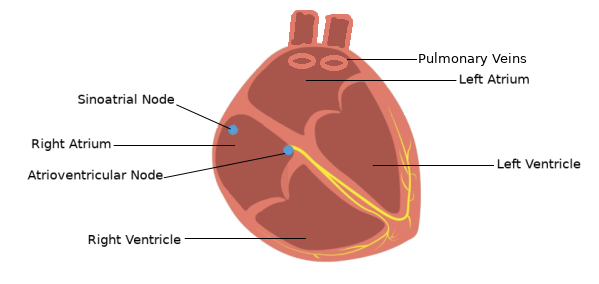
\includegraphics[width=\linewidth,trim=0 0.5cm 0 0,clip]{heart_diagram_withpvs}
	\caption{Simplified structure of the heart, as viewed from the front. Relevant anatomical features are indicated. The pulmonary veins are particularly relevant for atrial fibrillation~\cite{haissaguerre1998spontaneous, ehrlich2003cellular}. Adapted from~\cite{gary2016bayes}.}
	\label{fig:heartdiagram}
\end{mdframed} \end{figure}

\subsection{Action Potential and Signal Propagation}

The membrane potential is the potential difference across the cell membrane of a cardiomyocyte, defined such that positive charge flowing into the cell makes it more positive~\cite{nattel}. The cardiac action potential is a rapid change in the membrane potential due to charges moving across gap junctions between cardiomyocytes. This action potential is what causes the cardiomyocytes to contract, giving rise to the sinus rhythm~\cite{katz2010physiology}. 
A typical cardiomyocyte action potential is shown in Fig.~\ref{fig:atrialcap}, with various phases indicated:
\begin{itemize}
	\item Phase 4 is the resting state of the cell. In this phase the cell can be excited by a neighbouring cell.
	\item Phase 0 is the depolarisation or excitation of the cell, caused by the membrane potential reaching a certain `threshold potential'. The membrane potential typically reaches this threshold because of a neighbouring cell also depolarising. In this way an electrical signal can propagate through the heart by exciting connected cardiomyocytes which in turn excite their neighbours.
	\item Phases 1--3 are the refractory period of the cell. During this stage it cannot be excited. This ensures that the signal cannot double back; that is, if cell A excites cell B, then cell B cannot immediately excite cell A in return. This behaviour gives rise to a mostly united wavefront for an electrical signal propagating through the atrium.
\end{itemize}

An electrocardiogram measures the electrical activity of the heart using electrodes on the skin~\cite{pullan2005mathematically}. This is an indirect measure of the electrical signals propagating through the heart due to the cardiomyocyte action potential.
%An intra-cardiac electrogram (henceforth referred to as an electrogram) is an ECG with several additional leads inserted into the heart. Both of these are indirect measures of the electrical signals propagating through the heart due to the action potential of the cardiomyocytes.

\begin{figure}[h!] \begin{mdframed}
	\centering
	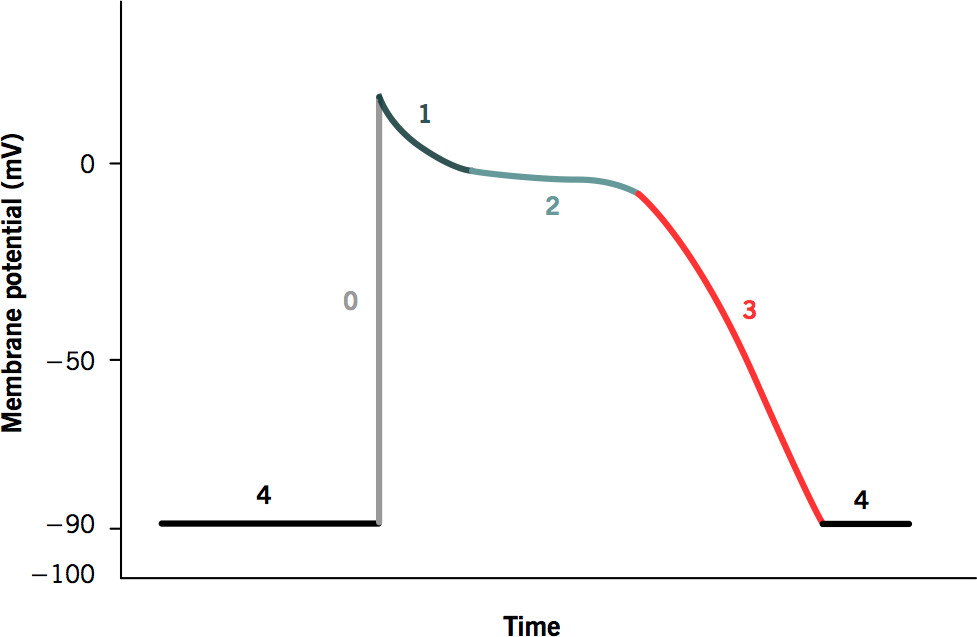
\includegraphics[width=0.7\textwidth]{action_potential_frompathophys.jpg}	
	\caption{A typical ventricular cardiomyocyte action potential, with phases indicated. In phase 0 the cell is said to be `excited' or `depolarised'. Phases 1--3 are the refractory period of the cell, during which it does not respond to electrical signals. In phase 4 the cell is resting and excitable. The `membrane potential' is the potential difference across the cell membrane, and is defined such that it becomes more positive as positive charge enters the cell~\cite{nattel}. Adapted from~\cite{pathophys}.}
	\label{fig:atrialcap}
\end{mdframed} \end{figure}

\section{Atrial Fibrillation}

Atrial fibrillation is a heart rhythm disorder characterised by an elevated heart rate and ineffective contraction of the atria. It results from sources of electrical signals outside the sinoatrial node.
An episode of atrial fibrillation may be categorised by its length:
\begin{itemize}
    \item Paroxysmal if it self-terminates within 7 days.
    \item Persistent if it lasts longer than 7 days but less than 12 months.
    \item Long-standing persistent if it lasts more than 12 months.
    \item Permanent if physicians have ceased attempts to restore normal heart rhythm~\cite{uptodate}.
\end{itemize}

\subsection{Mechanisms}

The precise mechanisms of AF are unknown, but several competing theories exist.

\subsubsection{Focal Ectopic Sources} 

These are rapidly repeating spontaneous excitations of individual cardiomyocytes outside of the sinoatrial node (usually seen in the pulmonary veins~\cite{uptodate, haissaguerre1998spontaneous}). These are thought to result from problems in the electrochemistry of individual cells. If these excitations repeat fast enough, the cell will take over control of the heart rhythm and induce AF~\cite{nattel}.
This theory has fallen out of favour as the primary maintainer of AF. However, it is believed that focal ectopic sources can initiate AF, as studies have shown that spontaneous cardiomyocyte excitations in the pulmonary veins may trigger the arrhythmia~\cite{haissaguerre1998spontaneous}.
	
\subsubsection{Re-entry Circuits}

Re-entry circuits are self-sustaining looping signals.
An `anatomical' re-entry circuit arises when a signal reaches an anatomical obstacle, such as a region of fibrosis, as illustrated in Fig.~\ref{fig:litreviewreentry}.

\begin{figure} \begin{mdframed}
    \centering
    \begin{subfigure}[b]{0.8\textwidth}
        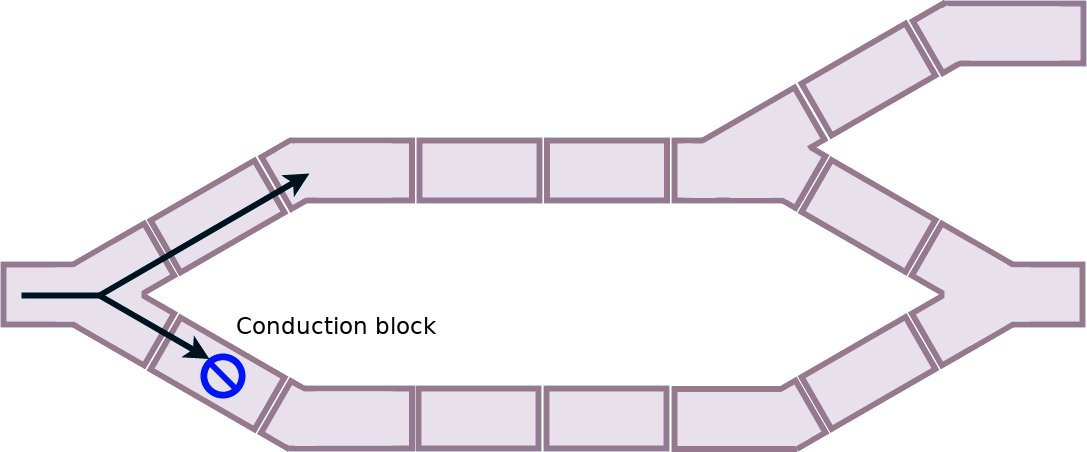
\includegraphics[width=\textwidth]{re_entry_formation_1}
        \caption{A signal enters from the cardiomyocyte on the left. It splits at the junction, and the signal on the upper branch continues while the signal on the lower branch is halted by some form of intermittent or unidirectional conduction block.  \\ }
    \end{subfigure}
    
    \begin{subfigure}[b]{0.8\textwidth}
        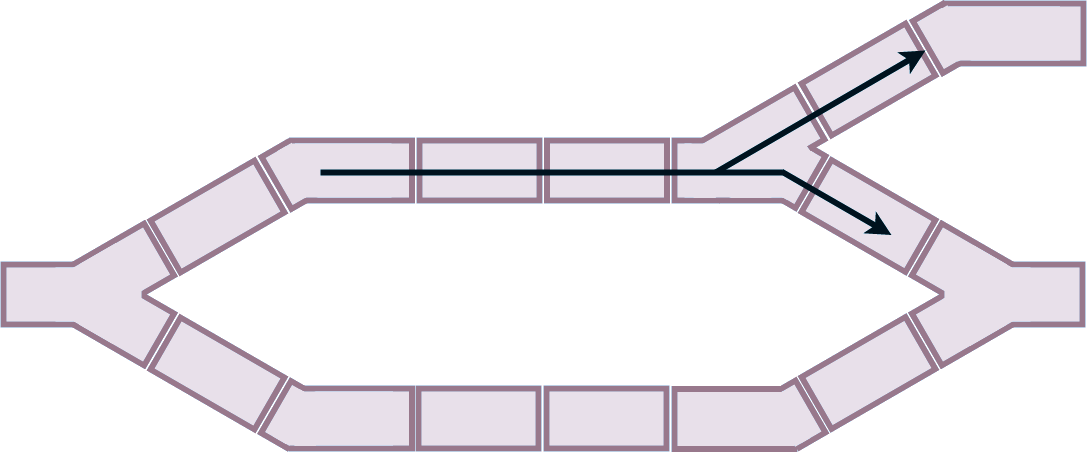
\includegraphics[width=\textwidth]{re_entry_formation_2}
        \caption{The signal continues to propagate on the upper branch, splitting at each junction it meets. \\ }
    \end{subfigure}
    
    \begin{subfigure}[b]{0.8\textwidth}
        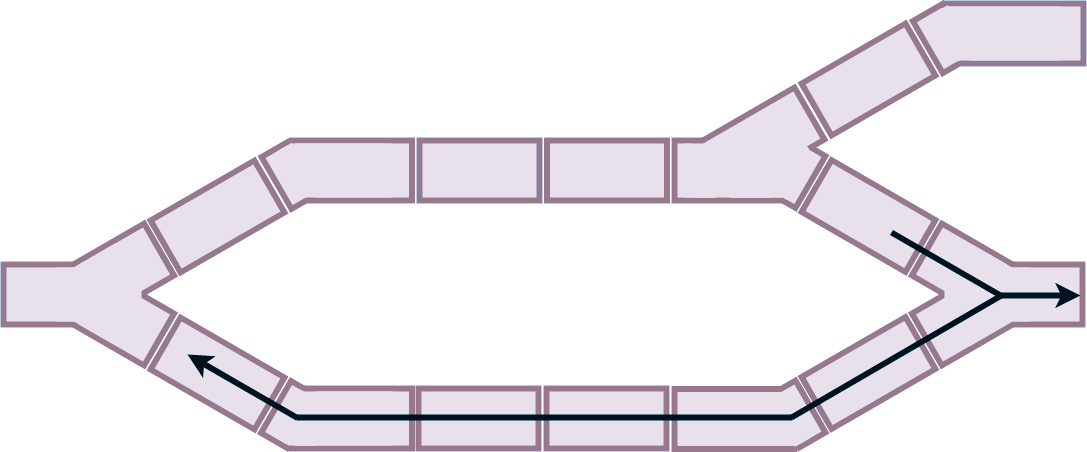
\includegraphics[width=\textwidth]{re_entry_formation_3}
        \caption{The signal ends up back on the lower branch, and passes through the conduction block. From here the signal will keep looping indefinitely.}
    \end{subfigure}
    \caption{Formation of an anatomical re-entry circuit. Each pink box represents a cardiomyocyte. The black arrowheads represent the wavefront of a signal, while their tails represent the refractory cells left in the wake of the signal. The large gap in the middle is an example of an anatomical obstacle.}
    \label{fig:litreviewreentry}
\end{mdframed} \end{figure}

The `refractory tail' (the refractory cells left in the wake of a signal) means that there is a minimum size for a re-entry circuit. Any smaller and the signal will collide with its own refractory tail and be extinguished. This minimum length is called the `wavelength of re-entry', and is given by product of the refractory period and conduction velocity~\cite{rensma1988length}. This explains why studies have found that decreasing the refractory period increased the risk of AF~\cite{rensma1988length}.

Functional re-entry is a re-entry circuit that forms around a `functional obstacle' rather than an anatomical obstacle. The nature of this functional obstacle varies between theories. For example, in `leading circle theory', the circuit generates a signal that propagates towards the centre of the circuit (as well as outwards), meaning that the centre of the circuit is composed of refractory tissue; the centre of the circuit therefore acts as a functional obstacle. Clinical observations incompatible with leading circle theory (namely that certain pharmacological treatments can reduce incidence of AF despite reducing the wavelength of re-entry) mean that this hypothesis has fallen out of favour~\cite{calkins2007hrs}.
`Rotors' are another hypothesised type of functional re-entry. In rotors, the centre of the circuit cannot be excited due to the high curvature of the part of the wave near the core~\cite{waks2014mechanisms} which lowers the speed of conduction due to the way a cell distributes current to its neighbours; the core therefore acts as a functional obstacle. Some studies purport to have found rotors in real hearts~\cite{Narayan1761}, but this is disputed~\cite{calkins2007hrs}.

A proposed resolution to the apparent discrepancy between focal and re-entrant drivers is that focal sources are not the primary driver, and are only observed due to limited resolution in surface mapping, only mapping one side of the heart, and complications from the way that re-entrant sources inside the heart project onto the surfaces~\cite{hansen}. Further research is needed to confirm or reject this hypothesis.
	
\subsection{Remodelling} \label{subsec:remodelling}

AF modifies the heart over time to make it a more favourable substrate for AF~\cite{wijffels1995atrial}. For example, sustained AF appears to promote fibrosis~\cite{burstein2007atrial, CORRADI20141250}, which in turn promotes AF~\cite{de2011fibrosis}. Additionally, if a cell is excited at a very high rate it will shorten its refractory period%
%in order to avoid an excessively high concentration of certain ions
~\cite{gaspo1997functional}, shortening the wavelength of re-entry and allowing more re-entry circuits to form. Both of these processes are examples of remodelling. In many cases paroxysmal AF progresses to persistent AF; remodelling provides one explanation for this~\cite{deVos2010progression}.

\subsection{Treatment}

The first line of treatment for AF is usually antiarrhythmic drugs, some of which work by lengthening the refractory period of the cardiomyocytes~\cite{bajpai2006atrial}. These are often used in combination with anticoagulants, as blood clots that form in the atria during AF can cause strokes~\cite{bajpai2006atrial}. However, antiarrhythmic drugs are not without risk and can themselves cause life-threatening rhythm disorders~\cite{nattel1998experimental}. Additionally, when used in the absence of surgical treatments, they only have a success rate of 16\%~\cite{wilber2010comparison}.

If pharmacological treatments for AF are unsuccessful, catheter ablation is used instead. This means using a catheter, inserted into a vein and guided to the heart, to surgically destroy or isolate regions of tissue responsible for AF. However, locating these regions is a difficult challenge. It has been found that 52\% of patients undergoing ablation experience no further episodes of AF, and a further 24\% experience no further episodes when using antiarrhythmic drugs as well as ablation~\cite{cappato2005worldwide}. In addition to this poor success rate, 6\% of ablation procedures have complications~\cite{deshmukh2013hospital}, which is why it is typically used only after antiarrhythmic drugs have failed.

As the pulmonary veins are a common substrate for both ectopic sources~\cite{haissaguerre1998spontaneous} and re-entry circuits~\cite{ehrlich2003cellular}, pulmonary vein isolation is a common ablation procedure involving electrically isolating the pulmonary veins from the rest of the atrium~\cite{calkins2007hrs}. 

Various methods have been proposed for determining regions to ablate~\cite{narayan2012treatment, nademanee2004new, hunter2011characterization, kottkamp2016box, miller2014initial, sommer2016successful} but they are generally unreliable or have failed to be reproduced in subsequent studies~\cite{calkins2007hrs, BUCH2016636, verma2015approaches, providencia2015there}. 
% Examples include isolating areas of high fibrosis, ablating areas which appear to show multiple deflections of electrical signals, and ablating rotors directly.

% \subsection{Mapping AF Drivers}

% A complex fractionated atrial electrogram is an electrogram that indicates multiple deflections of a propagating signal lasting longer than a particular length of time. A 2004 study found that ablating in areas showing these electrograms was effective at curing AF~\cite{nademanee2004new}. Later studies have failed to reproduce this effect~\cite{verma2015approaches, providencia2015there}, but one study found that particular classifications of complex fractionated atrial electrograms were a good indication of areas to ablate~\cite{hunter2011characterization}. Further study may be required.

% There are other novel methods for determining regions to ablate. Isolation of areas with high fibrosis in combination with pulmonary vein isolation has shown promising initial results~\cite{kottkamp2016box}. Ablation of rotors  showed promising initial results~\cite{narayan2012treatment, miller2014initial, sommer2016successful} but other studies have failed to reproduce these~\cite{BUCH2016636}.

\section{Modelling Atrial Fibrillation}

Due to the difficulties of studying AF in living patients, it is desirable to design models instead. Models give greater control over the parameters of the atria than would be possible in an experimental setting, and are not invasive. Some models of cardiac electrophysiology model the heart as a continuum with anisotropic conduction properties; these are extremely fast to simulate, but may not reproduce phenomena arising from interactions between cells. Others consider the behaviour of ion currents between cells, but these are so computationally intensive that simulating even a single heartbeat is slow~\cite{Butters20120067, harrild2000computer, zhaoperformance}.

A middle ground between these two modelling approaches is to use cellular automata. In a cellular automaton, cells on a lattice are treated as discrete units with a finite number of states. At each step of the model, the new state of each cell is determined by its own state and the state of other cells in its neighbourhood~\cite{wolfram1983statistical}. Cellular automata don't take into account the full complexities of the internal behaviour of cells or detailed interactions between them, so may not reproduce phenomena emerging from these more detailed interactions. Additionally, a cellular automaton cannot model long-term changes or rate-dependent effects~\cite{pullan2005mathematically}, such as remodelling.
Despite these limitations, the cellular automaton approach carries significant advantages. The cardiomyocytes are discrete and, under this approach, they are treated as such. The simplified nature of this approach also allows the model to run extremely fast, so large quantities of data can be collected for analysis. Cellular automata can still be useful even if the internal workings of the cardiomyocytes are not well-understood or are extremely difficult to simulate, as this detail is abstracted away.

\section{Key Points from Chapter \thechapter}

\begin{itemize}
    \item Atrial fibrillation is caused by abnormal behaviour of electrical signals in the heart; anatomical re-entry circuits are especially important in the upcoming chapters.
    \item Treatments for AF are ineffective and attempts to locate re-entry circuits have historically been disappointing.
    \item Fibrosis results in fewer connections between muscle fibres, and has been implicated in AF.
    \item The heart cells obey an action potential with three distinct phases: excited $\rightarrow$ refractory $\rightarrow$ resting. This behaviour allows electrical signals to be conducted through the atrium.
    \item Cellular automata are a natural choice when modelling the heart, and carry enormous speed advantages compared to more detailed models.
\end{itemize}

